% ...existing code...

\chapter{Infraestructura física y puesta a punto}

\section{Primer contacto con la infraestructura y proceso de instalación}
El comienzo de este proyecto arrancó con un primer contacto directo con el hardware: la puesta a punto del servidor \textit{Dell PowerEdge R7615} \cite{ref45} en las instalaciones del Centro de Transferencia Tecnológica de la UGR (CTT). Este proceso, fundamental para el desarrollo del trabajo, se realizó siempre bajo supervisión, asegurando el cumplimiento de los protocolos de seguridad y las prácticas técnicas establecidas por el centro.

% [Sala de servidores del CSIR]
\begin{figure}[H]
    \centering
    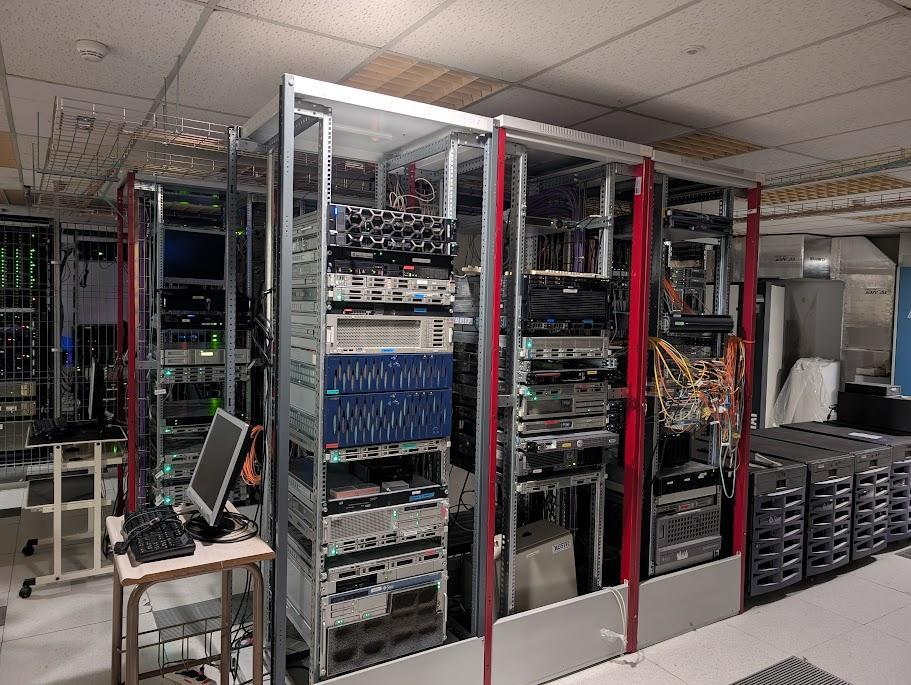
\includegraphics[width=0.6\textwidth]{imagenes/image47.jpg}
    \caption{Sala de servidores del CTT.}
    \label{fig:sala-csir}
\end{figure}

La instalación se formalizó mediante una solicitud de acceso detallando el porque de la visita, dado el control exhaustivo del centro sobre el acceso a la sala de servidores, un punto crítico para la información y el servicio universitario. El montaje se llevó a cabo en un rack estándar de 42U, respetando las distancias mínimas de ventilación ($\geq$30 cm por delante y por detrás) para garantizar una refrigeración óptima y evitar el sobrecalentamiento. Además, las instalaciones cuentan con un control riguroso de la temperatura para la protección de todos los servidores. Se configuraron dos fuentes de alimentación separadas y conexiones de red de alta velocidad de 10~Gbps, buscando asegurar la redundancia y la operatividad continua del sistema ante posibles fallos.

% [Dell PowerEdge R7615 en el rack]
\begin{figure}[H]
    \centering
    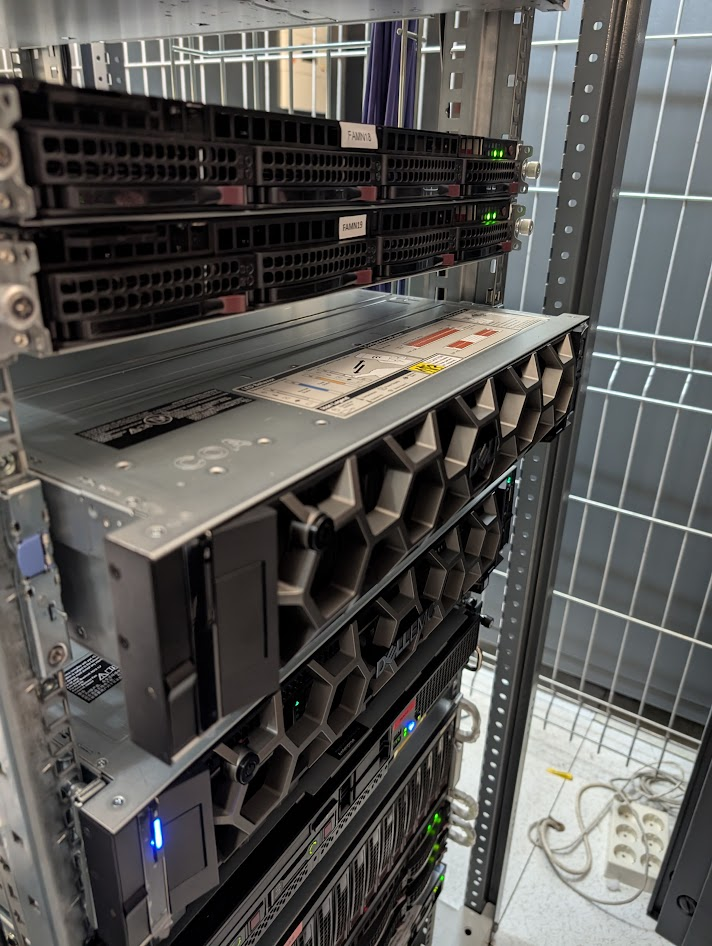
\includegraphics[width=0.5\textwidth]{imagenes/image56.png}
    \caption{Dell PowerEdge R7615 en el rack.}
    \label{fig:poweredge-r7615-rack}
\end{figure}

Fue curioso cómo un pequeño accidente hizo ver las cosas con otra perspectiva. Al desempaquetar el servidor, sin darse cuenta, se produjo un corte con el borde de la caja. Nada grave, pero el incidente, con el dedo sangrando en medio de la instalación, resultó impactante. Lo que impresionó fue la rapidez con la que el tutor sacó el botiquín de la sala para proporcionar una tirita, además de la disponibilidad de un cuarto de baño para limpiar la herida.
\newpage
Mientras se aplicaba la tirita, se reflexionó: por más que se configuren sistemas complejos y redundancias técnicas, lo que marca la diferencia es algo tan simple como tener una tirita a mano. El suceso hizo darse cuenta de que, por mucho que se planifiquen los grandes problemas técnicos, son esos pequeños imprevistos cotidianos los que pueden retrasar todo un proyecto.

Se comprendió que este enfoque completo, preocuparse tanto por lo pequeño como por lo grande, es justo lo que hace que un sistema realmente funcione en el mundo real. En el enfoque de \textit{Site Reliability Engineering} (\textit{SRE}) no solo importa implementar arquitecturas impresionantes, también cuenta tener ese instinto para detectar dónde podría surgir el problema más sencillo. A veces, la diferencia entre un sistema que se mantiene operativo y uno que falla está en esos pequeños detalles que parecen insignificantes pero que, cuando aparecen, pueden pararlo todo.

\begin{figure}[H]
    \centering
    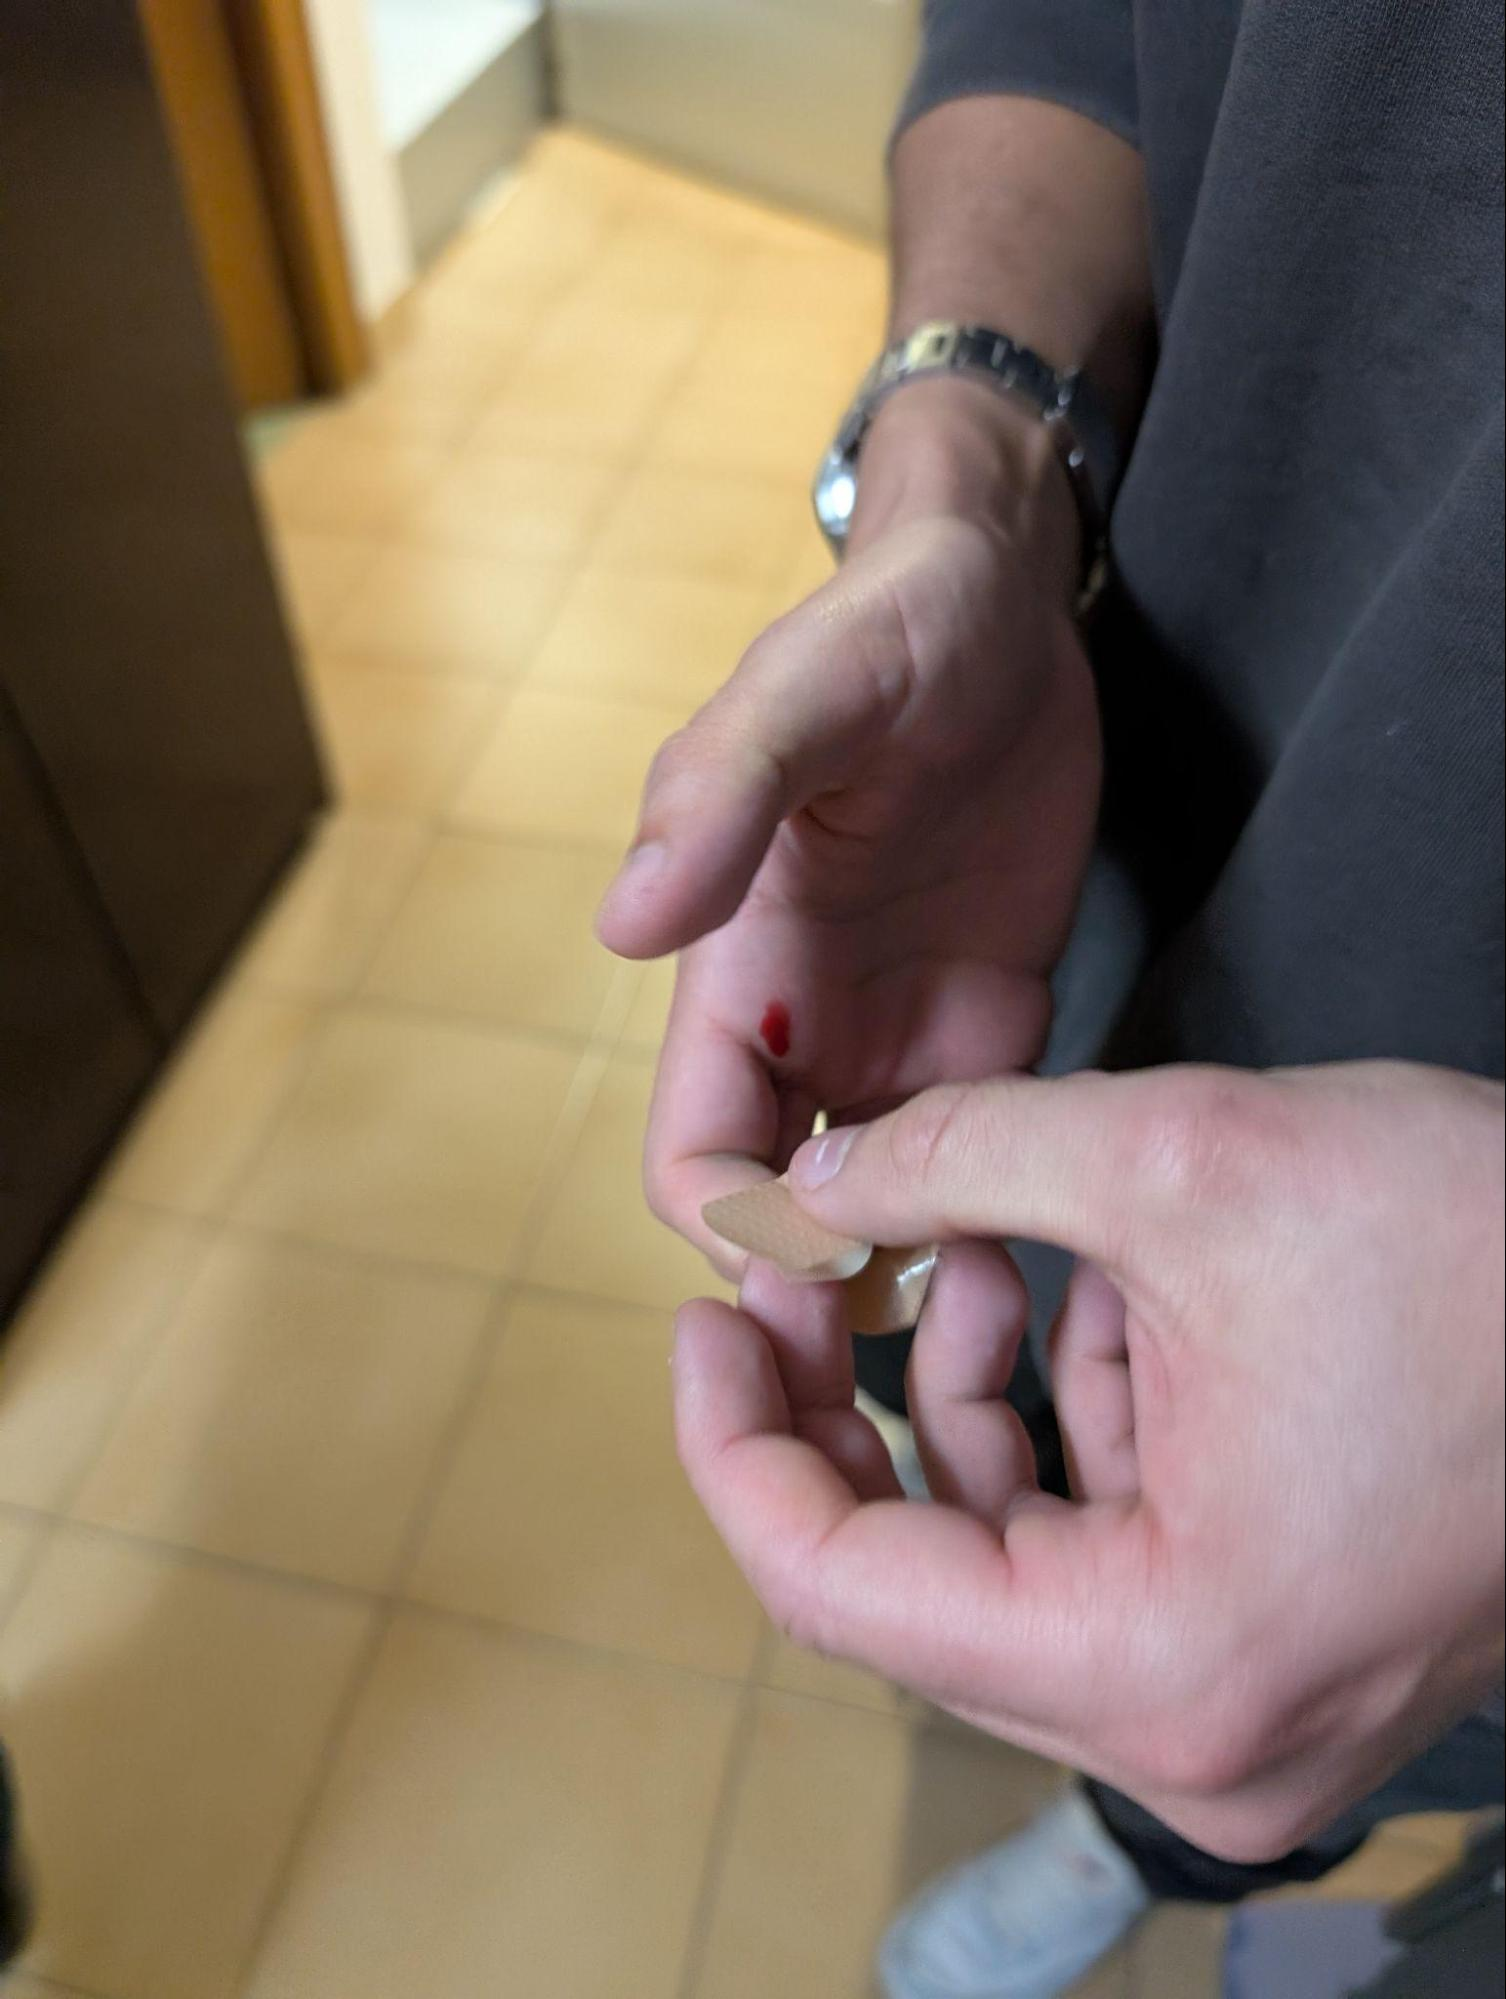
\includegraphics[width=0.5\textwidth]{imagenes/image4.jpg}
    \caption{Corte en el dedo.}
    \label{fig:corte-dedo}
\end{figure}

\newpage
\section{Experiencia con la Configuración de Servidores}
Para el servidor específico de este proyecto, la instalación del sistema operativo y el cableado principal fueron gestionados por el personal técnico del centro universitario. Sin embargo, la experiencia previa en configuración de infraestructuras en las prácticas permitió complementar este punto.

En el rol de \textit{IT Infrastructure} en \textit{Desion} \cite{ref38}, se asumió la responsabilidad del \textit{setup} de servidores para aplicaciones de \textit{IA}, incluyendo el montaje físico de componentes como CPU y GPU, y el cableado. Además, se proporcionó soporte en la automatización de infraestructura, se monitorizó el rendimiento y la disponibilidad de sistemas, se optimizó \textit{pipelines CI/CD} y se comprendió la importancia crítica de la documentación técnica durante las instalaciones. Para estas tareas, se adquirió experiencia en el uso de herramientas como \textit{Nagios} \cite{ref50} y \textit{Grafana} \cite{ref51}, y se perfeccionó el manejo de \textit{Docker} \cite{ref54} para el despliegue de servicios empresariales, como la herramienta de anotación de datos \textit{CVAT} \cite{ref53} con \textit{Traefik} \cite{ref52}.

Un ejemplo relevante de esta experiencia fue la instalación de Ubuntu 22.04 \textit{LTS} en dos servidores Supermicro. Esta tarea permitió comprender la importancia de las versiones \textit{Long Term Support (LTS)}, que garantizan actualizaciones de seguridad y estabilidad a largo plazo, frente a versiones más recientes que pueden presentar incompatibilidades. Se selecciona esta version ya que los proyectos de \textit{Machine Learning} manejados en estos servidores están compilados y optimizados para esta versión. La actualización a una versión posterior (como Ubuntu 24.04) habría implicado problemas de compatibilidad con bibliotecas críticas como \textit{CUDA} \cite{ref24} y \textit{PyTorch} \cite{ref55}, lo que habría requerido una actualización y recompilación de todos los proyectos de ML, atrasando todos los proyectos y comprometiendo dicha estabilidad. 

Otro ejemplo de puesta a punto de infraestructura ocurrió durante un desplazamiento a Schwechat (Austria), donde se participó en la instalación física de los servidores mostrados en la imagen posterior (véase la figura~\ref{fig:rack-schwechat}). En esta ocasión, no solo se colaboró en el montaje físico de los equipos en un rack estándar de 42U, sino también en la planificación y ejecución del cableado estructurado, tanto de red como de alimentación. El rack fue equipado con un panel de distribución de fibra óptica, dos servidores ASUS ESC4000A-E12 \cite{ref79}, cada uno con una \textit{CPU AMD EPYC} y cuatro \textit{GPUs NVIDIA L4}, un servidor \textit{Fujitsu}, un \textit{SAI APC} (Sistema de Alimentación Ininterrumpida) y un switch de red de alto rendimiento con conectividad de 10~Gbps. Todos los equipos se organizaron con gestores de cableado para facilitar el mantenimiento y asegurar una ventilación adecuada. En cuanto al sistema operativo, se instaló Ubuntu 22.04 \textit{LTS} en ambos servidores ASUS y en el Fujitsu. Cabe mencionar que se instalaron estos SO mediante \textit{Iventoy} \cite{ref49}, un \textit{PXE Boot}\footnote{PXE Boot (Preboot Execution Environment) es un método para arrancar un equipo a través de la red en lugar de desde un disco local.} que yo mismo desplegué para la empresa y que permitió automatizar la instalación de varios sistemas al mismo tiempo, incluyendo su propio \textit{autoinstall} \cite{ref73}.

Para asegurar la monitorización del sistema, se configuró \textit{Nagios} en el servidor Fujitsu, el cual actuó como nodo de control. Este monitorizó el estado de los otros dos mediante chequeos periódicos de disponibilidad, uso de recursos y estado de red. 

% [Supermicro as-4124gs-tnr-03-wa0004]
% [Otro supermicro con 2 GPU 3090]
% [Rack de Servidores de Schwechat (Austria)]

\begin{figure}[H]
    \centering
    \begin{minipage}{0.4\textwidth}
        \centering
        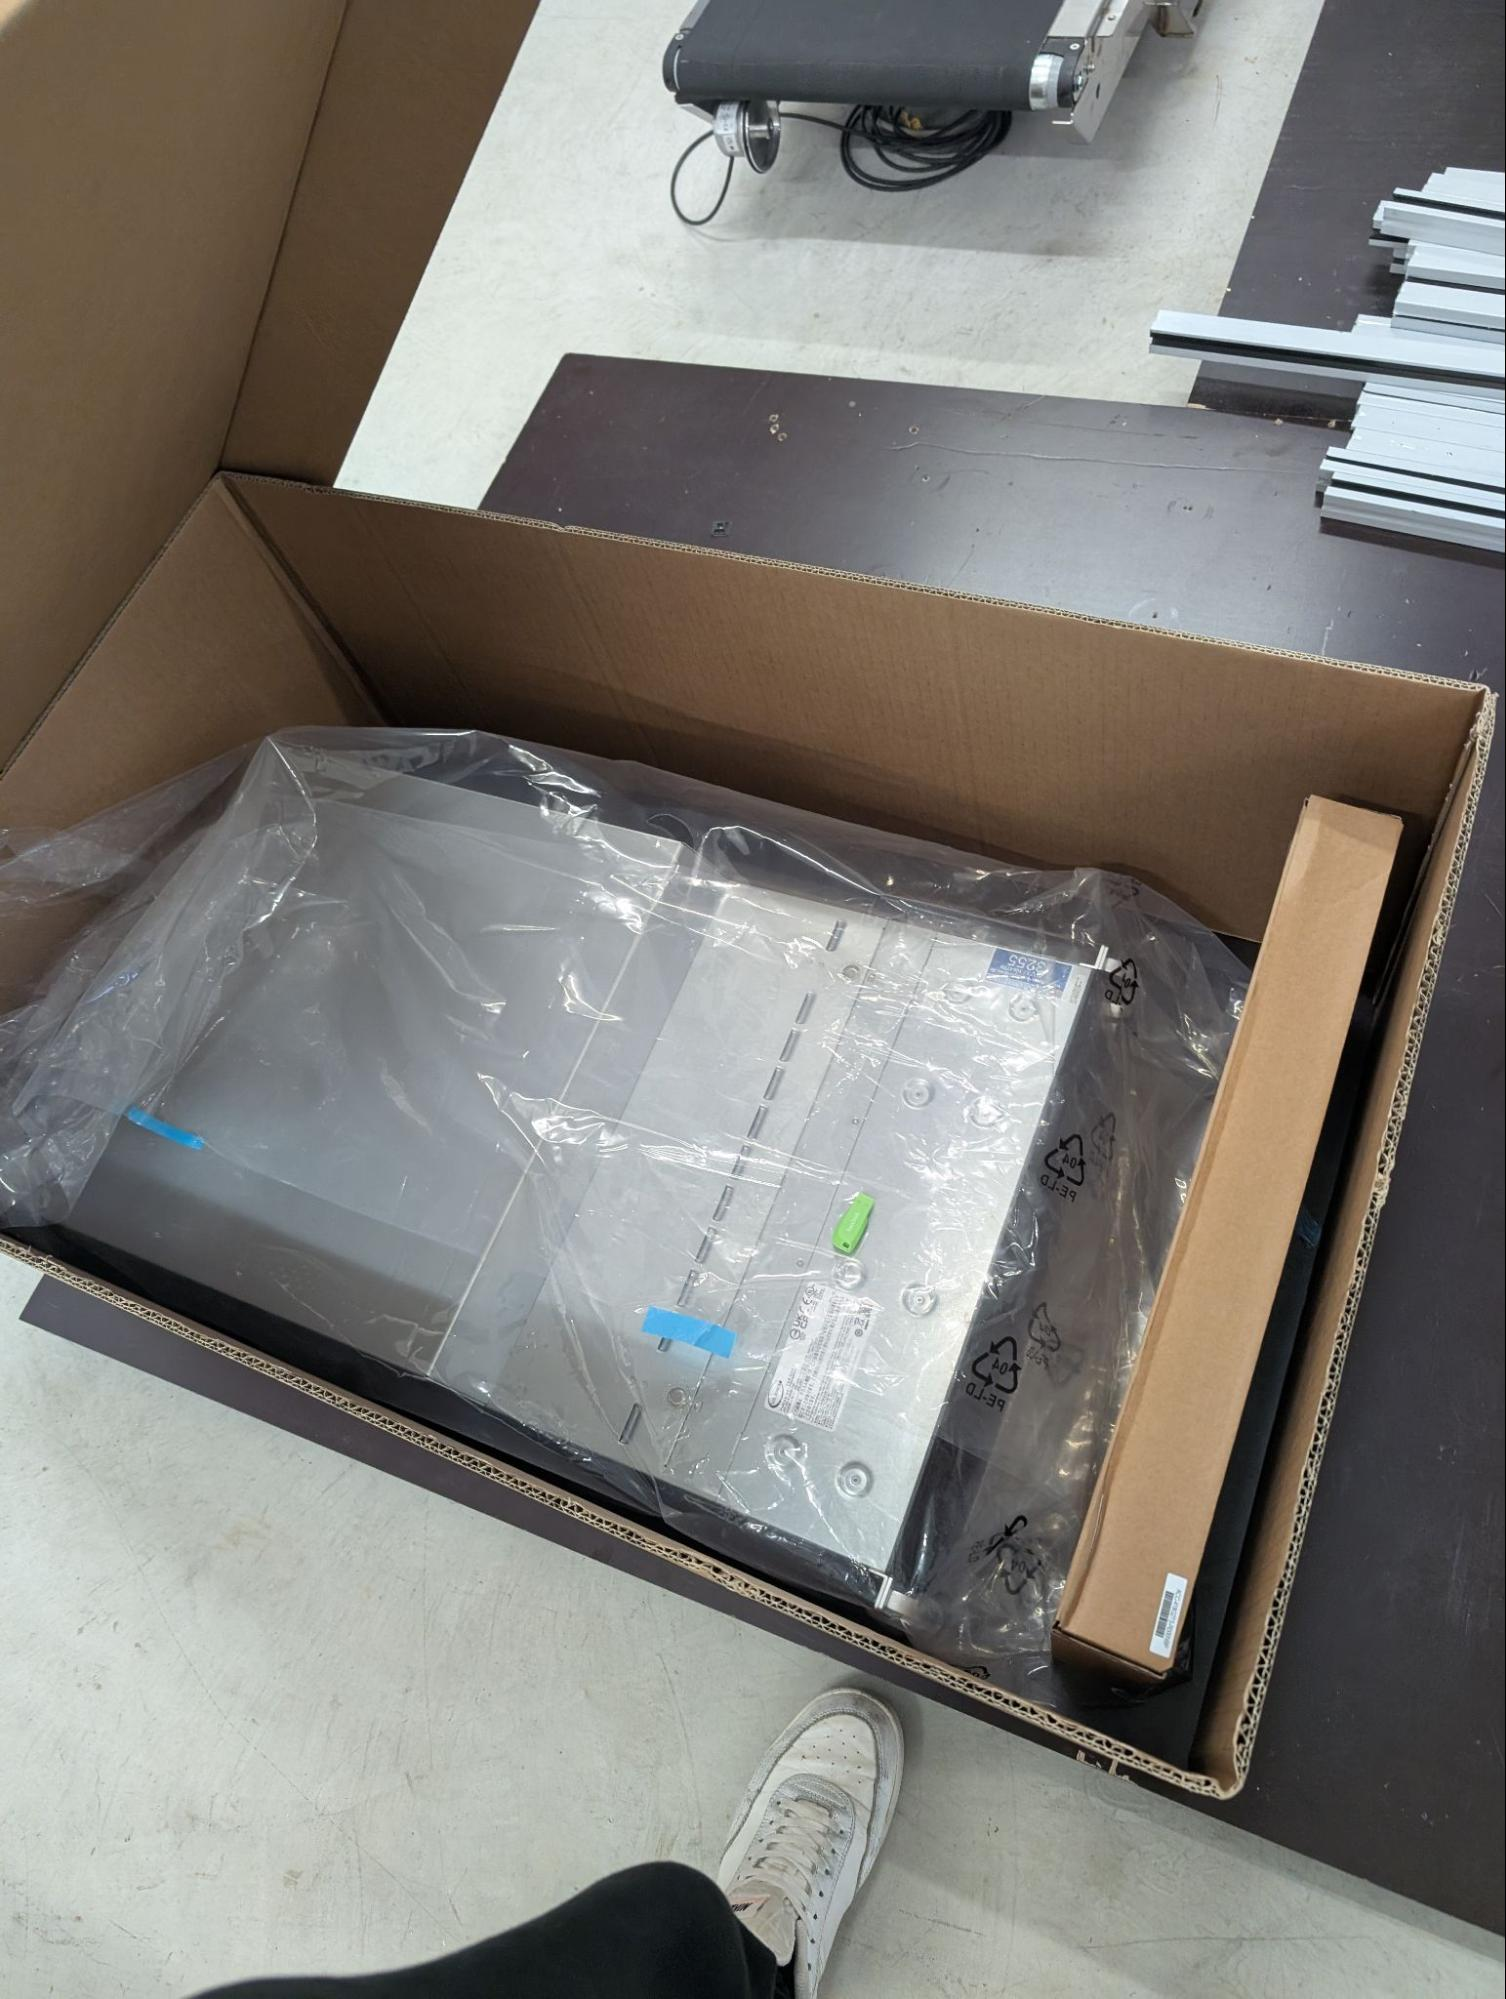
\includegraphics[width=\textwidth]{imagenes/image15.jpg}
        \caption{Supermicro as-4124gs-tnr-03-wa0004 en \textit{Desion} }
        \label{fig:supermicro-4124gs}
    \end{minipage}\hfill
    \begin{minipage}{0.4\textwidth}
        \centering
        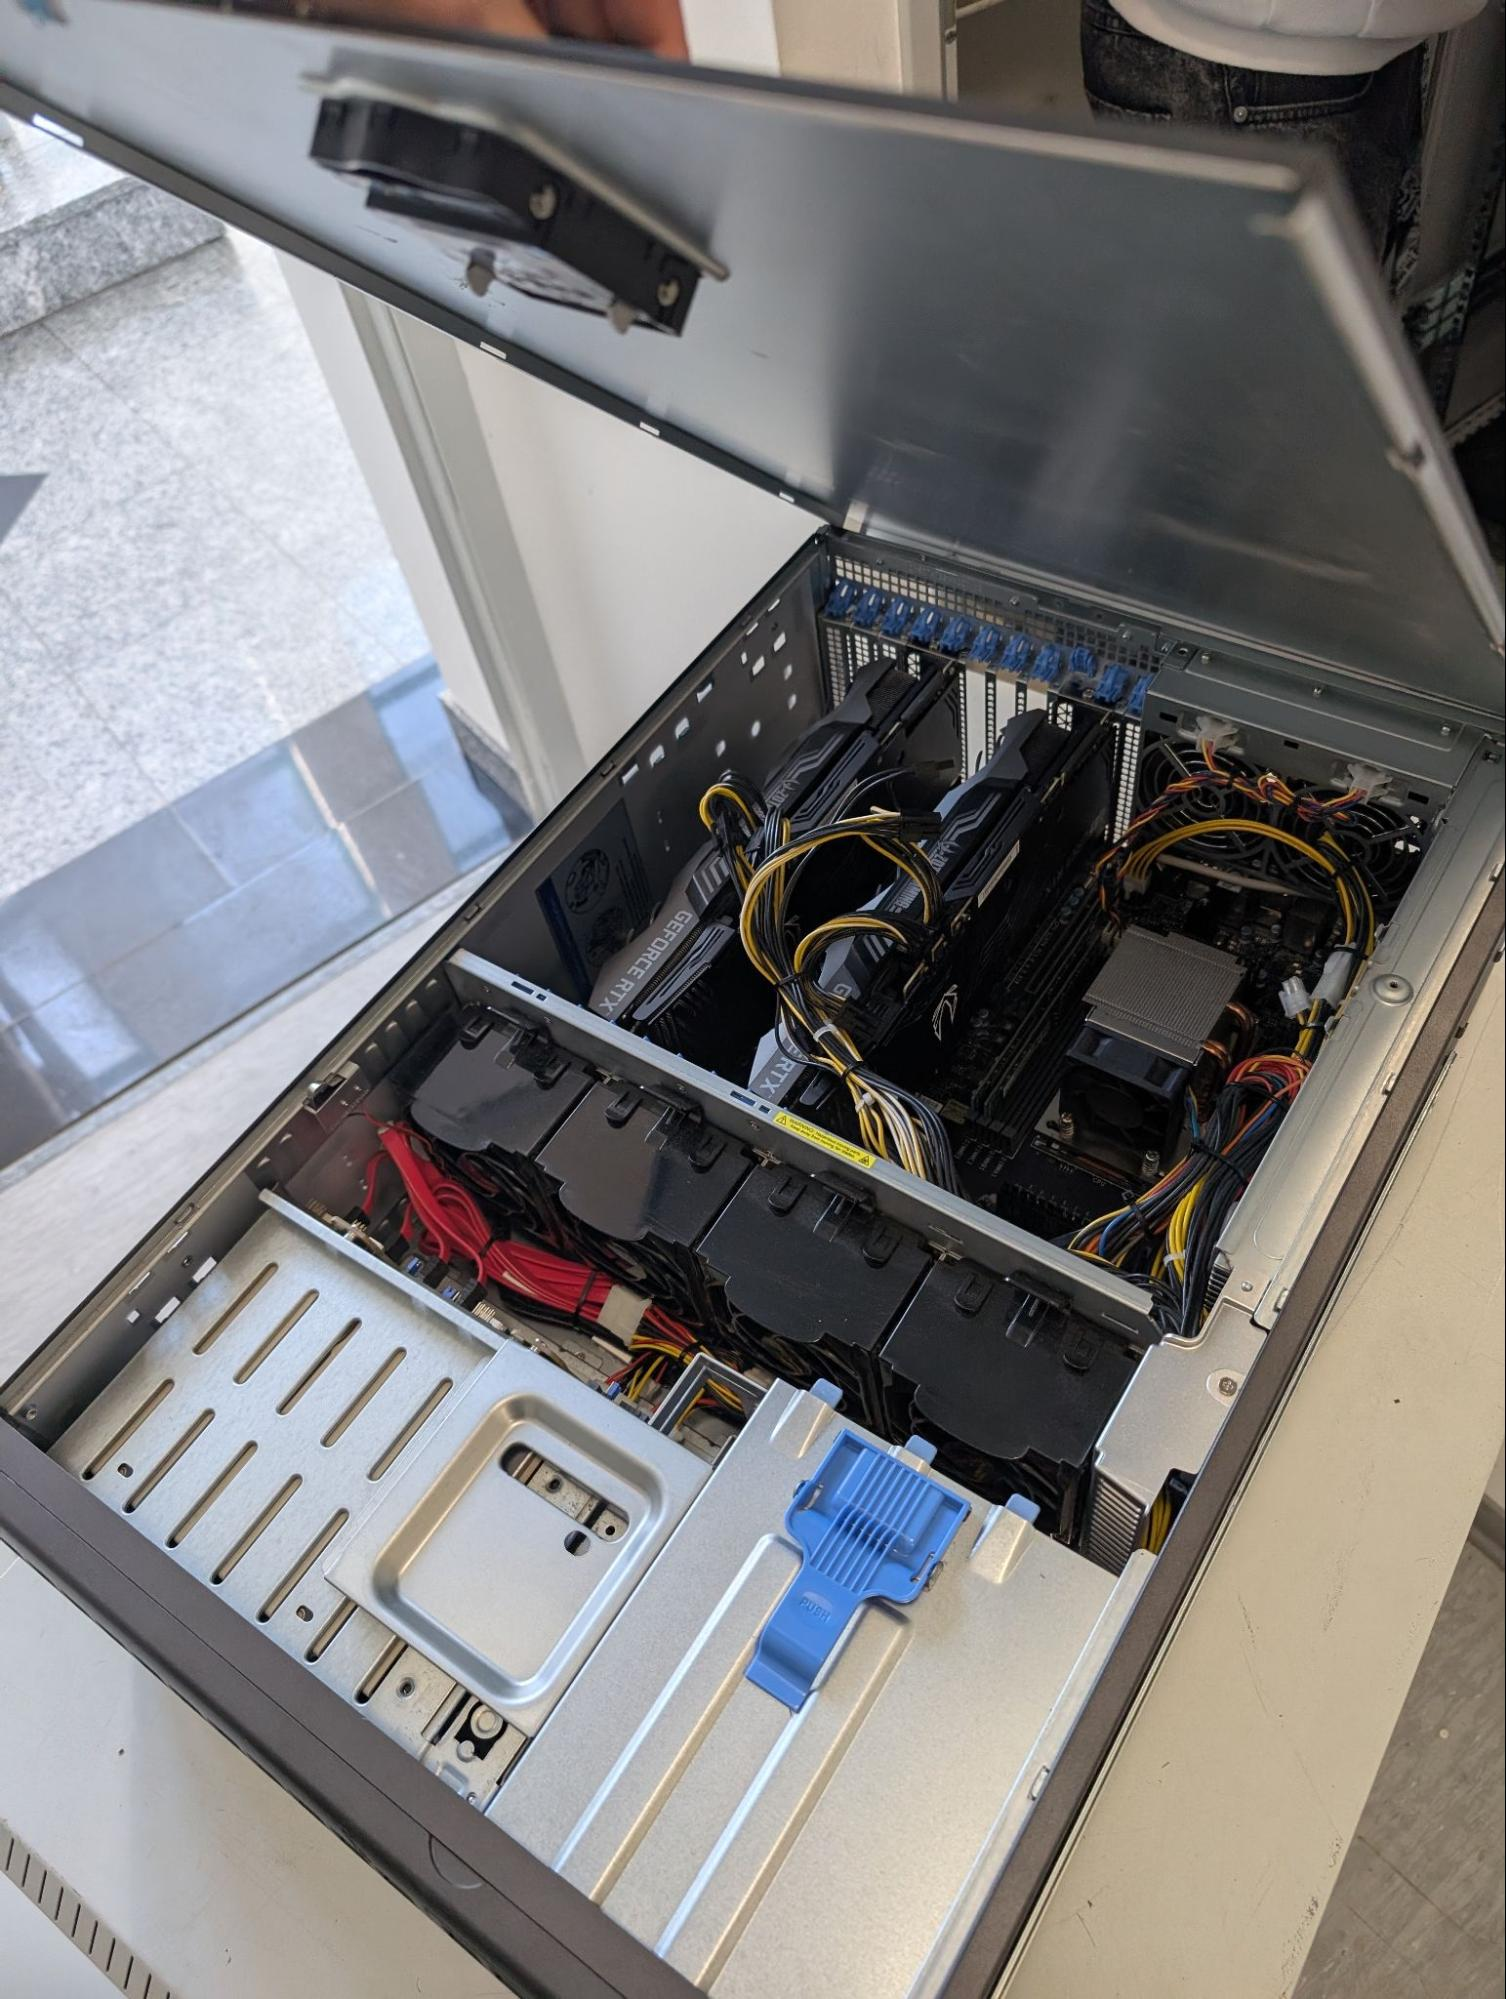
\includegraphics[width=\textwidth]{imagenes/image52.jpg}
        \caption{Otro supermicro con 2 GPU 3090 en \textit{Desion} }
        \label{fig:supermicro-2gpu3090}
    \end{minipage}
\end{figure}

\begin{figure}[H]
    \centering
    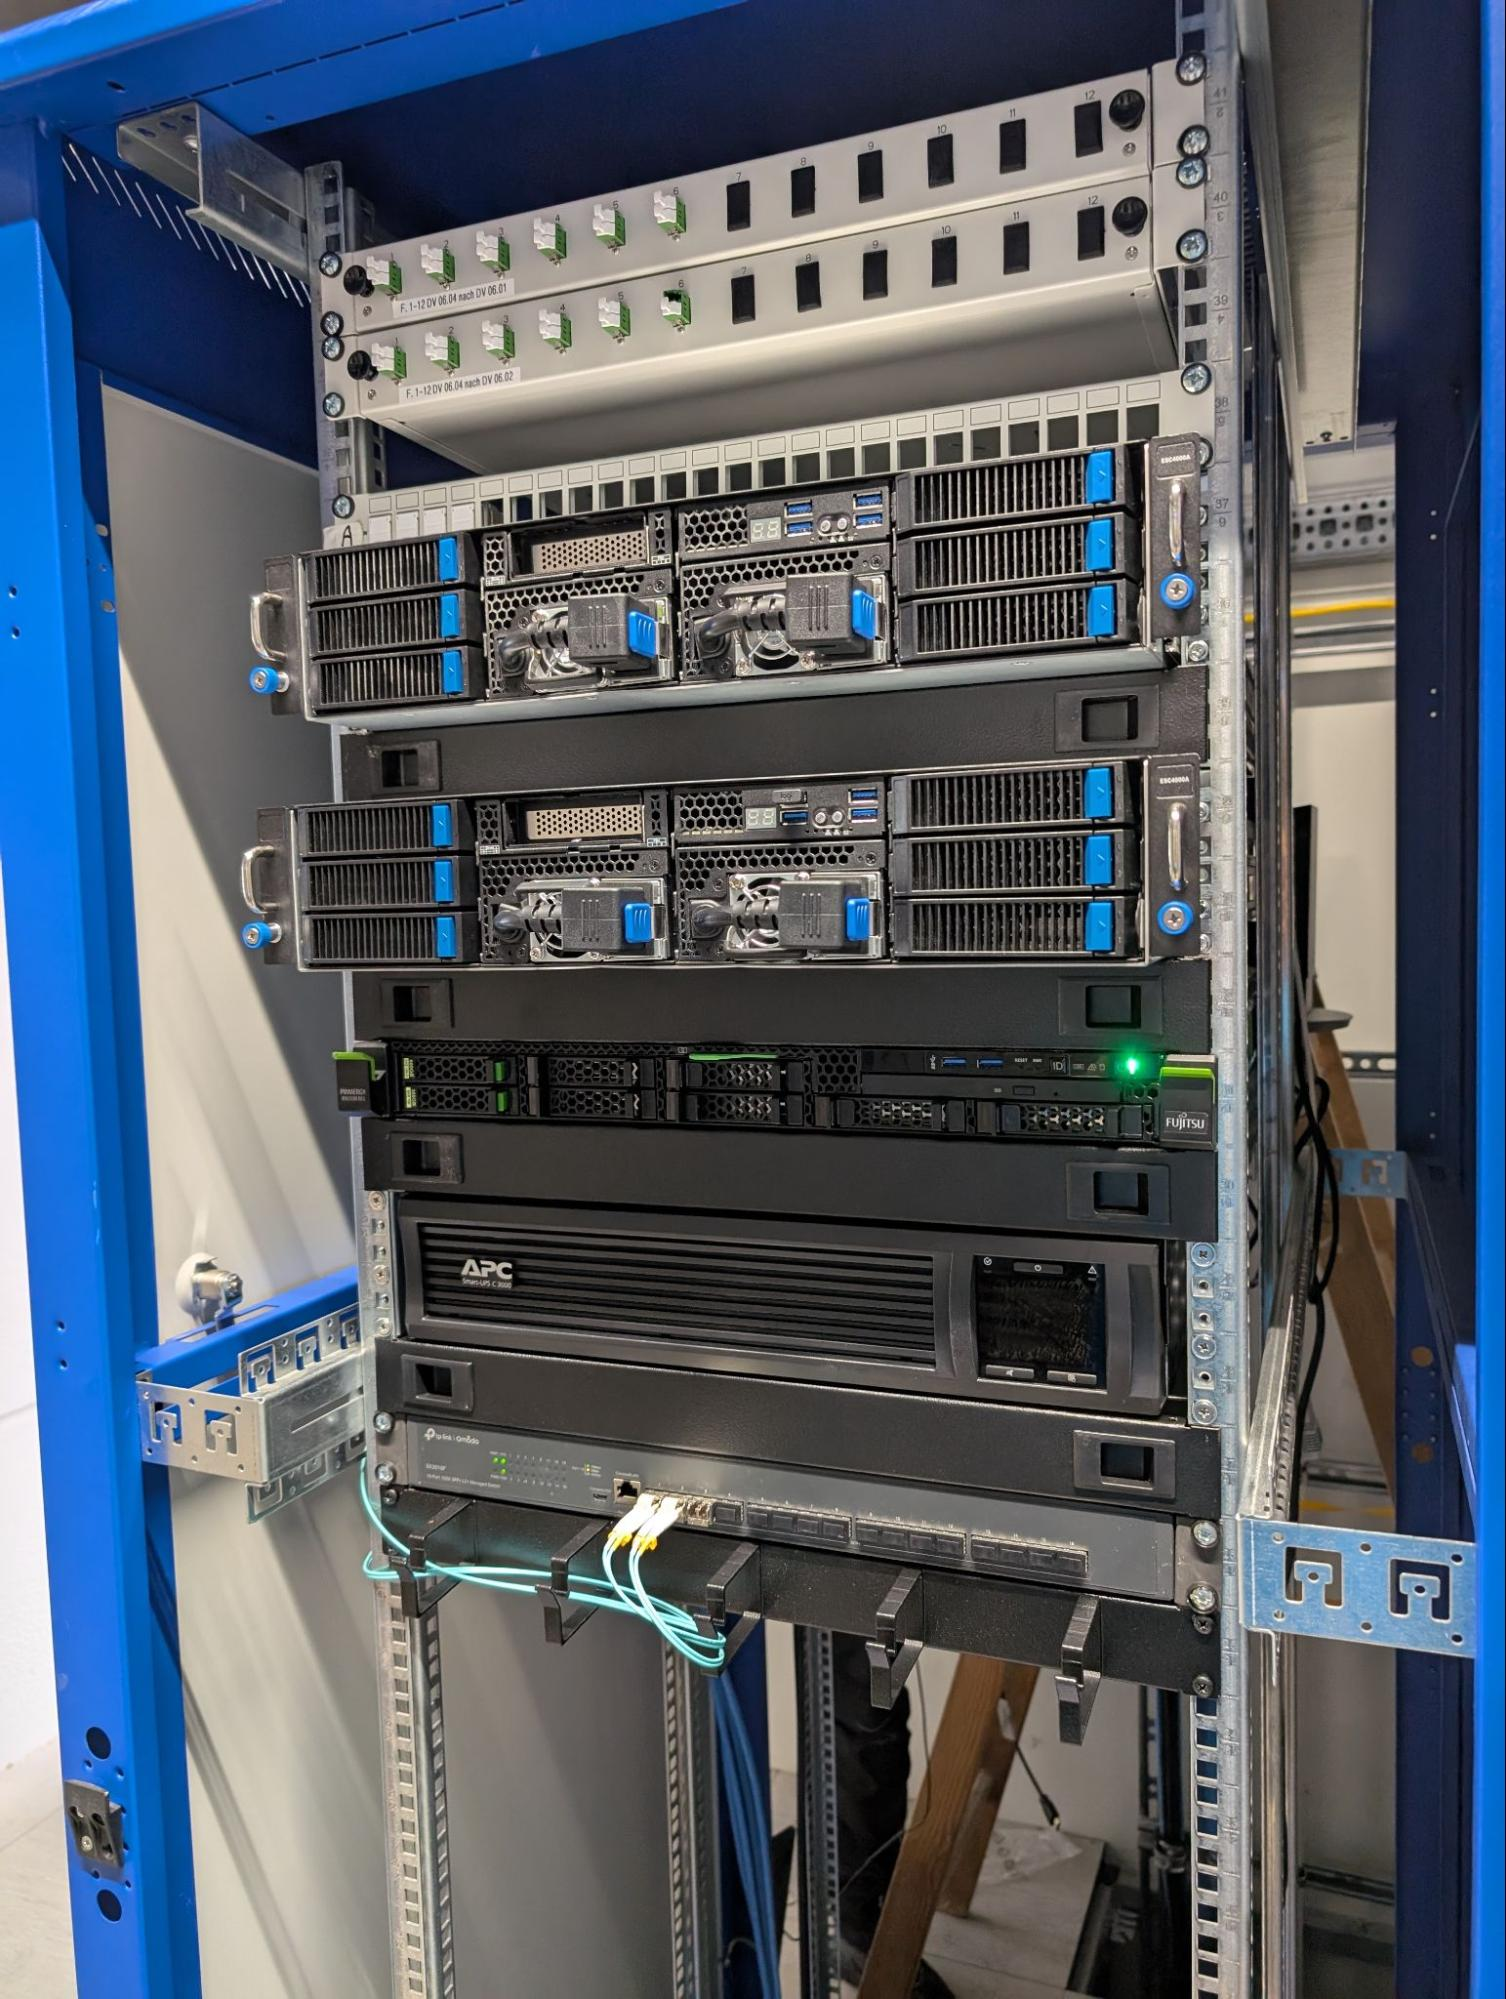
\includegraphics[width=0.4\textwidth]{imagenes/image17.jpg}
    \caption{Rack de Servidores de Schwechat (Austria)}
    \label{fig:rack-schwechat}
\end{figure}


\section{Conexión Remota y Acceso al Servidor}
El manejo del servidor, ubicado en la Universidad de Granada (España), se realizó de forma remota desde Darmstadt (Alemania). Esta situación exigió una conexión remota para el desarrollo del \textit{TFG}.

Fue importante reconocer que el acceso remoto es un punto crítico de seguridad en cualquier infraestructura. Por ello, siempre se recomendó aplicar principios como la restricción de privilegios, la trazabilidad mediante auditorías y la automatización, cuando sea posible. Esto minimiza errores humanos y aumenta la resiliencia operativa.

Aunque se intentó una conexión directa vía \textit{VPN}, problemas de configuración en el servidor principal impidieron esta opción. Por ello, se optó por una alternativa que requirió dos saltos de conexión: el primero a una máquina intermedia (máquina-A) y el segundo al servidor objetivo (máquina-B). Por motivos de seguridad, y para proteger información sensible, los nombres de host y usuarios específicos se omiten en esta documentación. La metodología de conexión se detalla a continuación.

Para el acceso se empleó \textit{SSH (Secure Shell)}, un protocolo estándar que cifra la comunicación en red. Aunque el puerto por defecto de \textit{SSH} es el 22, su uso predeterminado lo convierte en un objetivo frecuente de ataques automatizados, como los de fuerza bruta. Utilizar puertos no estándar, como el usado en el servidor principal en este caso para el segundo salto de conexión, redujo la exposición directa a estos escaneos y aumentó la seguridad.

\subsection*{Pasos para la Conexión Remota}
La conexión se estableció primero con una máquina intermedia de la Universidad de Granada. El comando utilizado fue:
\begin{verbatim}
ssh user@maquina-a
\end{verbatim}

Desde la máquina intermedia, se accedió al servidor \textit{HPC}. En este caso se abrió un puerto específico para entrar al servidor como se menciona anteriormente. El comando fue:
\begin{verbatim}
ssh maquina-b -p XXXXX -vvv
\end{verbatim}

Aquí, \texttt{-p} especificó un puerto no estándar por motivos de seguridad. La opción \texttt{-vvv} mostró información detallada de la conexión, lo cual fue importante para depurar problemas. Se utilizó principalmente al intentar conectar directamente con la \textit{VPN} de la universidad activa, lo que permitió identificar que la \textit{VPN} no estaba realizando el \textit{tunneling} correctamente porque el servidor no estaba configurado para ello.

\subsection*{Configuración de Autenticación por Clave SSH}
Para simplificar y asegurar el acceso, se automatizó el proceso mediante autenticación por clave \textit{SSH} en lugar de contraseñas, lo que evitó la necesidad de introducir credenciales múltiples veces. Este método se aprendió y aplicó muchas veces durante las prácticas \textit{Erasmus}, dado que en la oficina el manejo de servidores siempre se realizó a través de \textit{SSH}. También en la oficina era común el uso de \textit{Xorg} con \textit{Remote Desktop} para una conexión con interfaz pero este no era el caso. La autenticación por clave mejoró significativamente la seguridad al eliminar el riesgo de ataques de fuerza bruta basados en contraseñas y la exposición de credenciales, además de automatizar el acceso. Este procedimiento se realizó con la autorización del tutor.

El proceso comenzó con la generación de un par de claves \textit{SSH} en la máquina local. Se recomendó el algoritmo \textit{ed25519} \cite{ref56} por su seguridad y eficiencia, siendo un algoritmo de criptografía de curva elíptica moderno que se ha vuelto muy recomendado y cada vez más utilizado para claves \textit{SSH}. El comando para generar la clave fue:
\begin{verbatim}
ssh-keygen -t ed25519 -C "correo-usuario"
\end{verbatim}

Aquí, \texttt{-t ed25519} definió el tipo de clave como un algoritmo moderno y seguro, y \texttt{-C} permitió añadir un comentario, como un correo electrónico, para identificar la clave. La passphrase pudo dejarse vacía si no se requería una capa adicional de seguridad. La clave pública (\texttt{id\_ed25519.pub}) y la privada (\texttt{id\_ed25519}) se guardaron en el directorio \texttt{~/.ssh/}.
Luego, la clave pública se copió a la máquina intermediaria para establecer la confianza, empleando:
\begin{verbatim}
ssh-copy-id user@maquina-a
\end{verbatim}
para una transferencia rápida y segura. A continuación, la misma clave pública se copió al servidor \textit{HPC} (máquina B). Se debió reemplazar \texttt{mi-clave} con el texto exacto del archivo \texttt{~/.ssh/id\_ed25519.pub}. El comando para esto fue:
\begin{verbatim}
echo "ssh-ed25519 mi-clave" | ssh -p 24134 user@maquina-b "mkdir -p ~/.ssh;\
 cat >> ~/.ssh/authorized_keys; chmod 700 ~/.ssh;\ chmod 600 ~/.ssh/authorized_keys"
\end{verbatim}

Este comando aseguró que los directorios y archivos tuvieran los permisos adecuados para la seguridad de \textit{SSH}.
La verificación de la conexión final se realizó con:
\begin{verbatim}
ssh -J user@maquina-a user@maquina-b -p XXXX
\end{verbatim}

La opción \texttt{-J} utilizó la máquina A como salto intermedio para llegar a la máquina B.

\subsection*{Configuración del Archivo ~/.ssh/config}
Para simplificar la conexión y evitar comandos largos, se editó el archivo de configuración \textit{SSH} en la máquina local (\texttt{~/.ssh/config}) añadiendo las siguientes entradas:
\begin{verbatim}
Host maquina-a
    HostName maquina-a
    User user

Host maquina-b
    HostName maquina-b
    User user
    Port XXXXX
    ProxyJump maquina-a
\end{verbatim}
Con esta configuración, se logró conectar al servidor simplemente con el comando:
\begin{verbatim}
ssh maquina-b
\end{verbatim}

\begin{verbatim}
1 dispositivo tiene una actualización disponible.
Ejecute `fwupdmgr get-upgrades` para más información.

Last login: Fri Apr  4 16:43:37 2025 from XXX.XXX.XXX.XXX
[user@maquina-b ~]$
\end{verbatim}

Este proceso de autenticación basada en claves y configuración optimizada minimizó la intervención manual y redujo la complejidad del acceso, permitiendo centrar los esfuerzos en las tareas del proyecto.

\begin{figure}[H]
    \centering
    
\includegraphics[width=1\textwidth]{imagenes/diagrama.png}
    \caption{Diagrama del doble salto de conexión.}
    \label{fig:diagrama-infraestructura}
\end{figure}


\newpage
\section{Especificaciones del Servidor}
Tras establecer la conexión con el servidor, se procedió al estudio de la infraestructura con la que se trabajó. Para comprender los componentes que la forman, se utilizó un comando resumen (\textit{neowofetch}) \cite{ref57} que permitió visualizar las especificaciones más relevantes.

\begin{figure}[H]
    \centering
    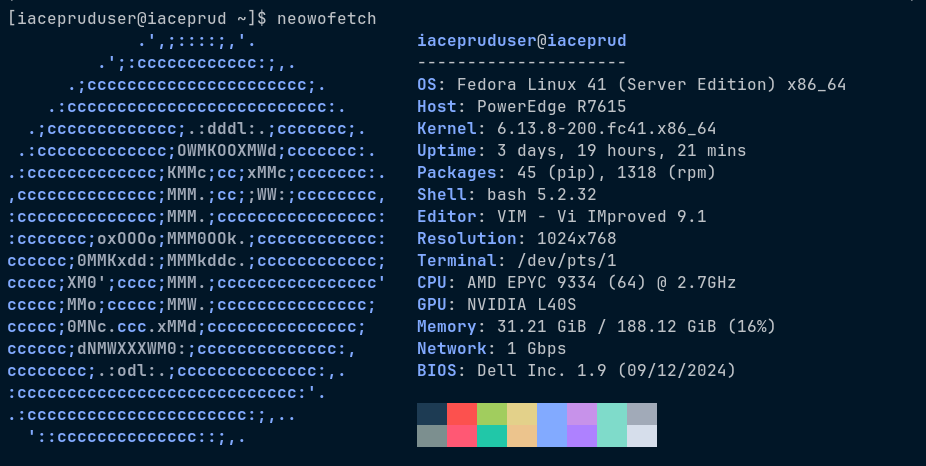
\includegraphics[width=0.9\textwidth]{imagenes/image1.png}
    \caption{Información del sistema (Neowofetch).}
    \label{fig:neofetch-info}
\end{figure}

\subsection*{Sistema Operativo}
El servidor utilizó \textit{Fedora Linux 41} en su edición para servidores, una distribución robusta y actualizada diseñada para entornos empresariales, que ofreció estabilidad. Su arquitectura es \textit{x86\_64}, compatible con procesadores de 64 bits y optimizada para tareas que requieren gran capacidad de cómputo. El kernel empleado fue la versión 6.13.8-200.fc41.x86\_64, una versión reciente que incorporó mejoras en seguridad, soporte de hardware y optimizaciones de rendimiento. También es importante resaltar su compatibilidad con la instalación de \textit{OpenShift}, \textit{Fedora} es propiedad de \textit{Red Hat}.

\subsection*{Procesador (CPU)}
El procesador instalado fue un \textit{AMD EPYC 9334}, basado en la arquitectura \textit{Zen 4} de la serie \textit{EPYC 9004}. Este modelo destacó por su eficiencia energética y su capacidad para procesamiento paralelo, características ideales para servidores. Aunque el \textit{EPYC 9334} tiene 32 núcleos y 64 hilos por socket, el sistema mostró 64 núcleos físicos, lo que sugirió la presencia de dos sockets, elevando la capacidad total a 64 núcleos y probablemente 128 hilos. Esto lo convirtió en una unidad muy potente para tareas multinúcleo. Su frecuencia base es de 2.7 GHz, con capacidad para aumentar mediante \textit{turbo} bajo demanda, optimizando el rendimiento en momentos de alta carga.

\subsection*{Memoria RAM}
El sistema dispuso de 188.12 GiB\footnote{GiB (Gibibyte) es una unidad de medida de almacenamiento equivalente a $2^{30}$ bytes, es decir, 1\,073\,741\,824 bytes. Se diferencia del GB (Gigabyte), que equivale a $10^9$ bytes.} de memoria RAM, utilizando tecnología DDR5 con corrección de errores (\textit{ECC}), un estándar en servidores que aseguró la integridad de los datos y soportó aplicaciones intensivas en memoria. En el momento del análisis, solo el 16\% de esta capacidad estaba en uso (equivalente a 31.21 GiB), lo que dejó un amplio margen para manejar cargas adicionales sin comprometer el rendimiento, indicando una configuración bien adaptada a las tareas actuales.

\subsection*{Unidad de Procesamiento Gráfico (GPU)}
El servidor estuvo equipado con una \textit{NVIDIA L40S}, una GPU de alto rendimiento diseñada para tareas avanzadas como inteligencia artificial, aprendizaje profundo, renderizado y computación científica. Esta unidad complementó la capacidad del servidor al ofrecer potencia adicional para procesamiento paralelo y aplicaciones que requieren cálculos gráficos intensivos, lo que la hizo ideal para entornos que demandan un alto nivel de cómputo más allá de las capacidades de la CPU. Escencial para el despliegue de \textit{LLM}.

\subsection*{Red}
Para examinar las interfaces de red, se utilizó el siguiente comando:
\begin{verbatim}
lspci | grep -i ethernet
\end{verbatim}

El sistema cuenta con múltiples interfaces de red Broadcom NetXtreme, incluyendo dos controladoras 10G RDMA Ethernet. Estas proporcionaron alta velocidad de transmisión y baja latencia, aspectos fundamentales para mantener la disponibilidad y la fiabilidad del sistema.


\newpage
\section{Clasificación de la Infraestructura como HPC}
Tras conocer en detalle las especificaciones del servidor, surgió la cuestión de si la infraestructura podía ser clasificada como un sistema (\textit{HPC}).

Según Dongarra en su estudio \textit{High-Performance Computing: Clusters, Constellations, MPPs, and Future Directions}~\cite{ref20} un sistema \textit{HPC} se caracteriza por la integración de múltiples nodos de cómputo interconectados, formando clústeres que permiten la ejecución paralela de aplicaciones a gran escala. Estos sistemas emplean herramientas específicas como \textit{MPI (Message Passing Interface)} y gestores de recursos como \textit{SLURM} \textit{(Simple Linux Utility for Resource Management)} para coordinar y optimizar las tareas distribuidas.

En este contexto, la infraestructura analizada, aunque equipada con hardware potente como el servidor Dell PowerEdge R7615, el procesador AMD EPYC 9334 y la GPU NVIDIA L40S, no cumple completamente con los criterios de un sistema \textit{HPC} completo. La ausencia de un clúster distribuido con múltiples nodos y la falta de herramientas de gestión específicas como \textit{MPI} o \textit{SLURM} limitan su clasificación como tal. La RAM de 188 GiB DDR5 con \textit{ECC} aseguró un manejo eficiente de grandes volúmenes de datos. Aunque dispuso de interfaces de red de hasta 10Gbps, operó con una conexión de 1~Gbps, suficiente para un nodo aislado, pero limitada para un entorno \textit{HPC} distribuido.

Por lo tanto, basándose en las definiciones y criterios establecidos en la literatura científica, la infraestructura descrita pudo considerarse un nodo de alto rendimiento preparado para tareas intensivas, pero no un sistema \textit{HPC} completo.

Sin embargo, el uso de herramientas de orquestación como \textit{OpenShift} permitió desplegar servicios, simulando parcialmente el comportamiento y la gestión de cargas típico de un entorno \textit{HPC}. A través de esta plataforma, fue posible automatizar la asignación de recursos, escalar servicios y supervisar el rendimiento del sistema, características clave en arquitecturas distribuidas. Aunque la infraestructura se limitó a un único servidor, la experiencia de operar en este entorno proporcionó una aproximación práctica al modelo \textit{HPC}.

Además, cabe destacar que para un estudiante, la gestión directa de una infraestructura \textit{HPC} representa una responsabilidad significativa, normalmente reservada para profesionales, sin embargo, este proyecto constituyó un primer paso fundamental. Poder trabajar con este tipo de servidor fue un privilegio, el cual permitió comprender en profundidad los fundamentos del cómputo de alto rendimiento.

Desde la perspectiva del \textit{Site Reliability Engineering}, conocer en detalle estas especificaciones no fue solo una cuestión informativa, sino una parte integral de la construcción de sistemas resilientes. Tal como se recomienda en las buenas prácticas de \textit{SRE} \Cite{ref6}, disponer de visibilidad clara sobre la infraestructura permite anticipar problemas como cuellos de botella, planificar escalabilidad y establecer mecanismos de recuperación más eficaces.


%Finalmente, fue importante conocer los recursos que se manejaron en la máquina para evaluar adecuadamente los servicios que se pretendieron desplegar en el futuro.

\newpage
\section{Instalación de los Controladores NVIDIA}
Se asignó la responsabilidad de instalar los controladores \textit{NVIDIA} en el servidor, el cual se compartía con otros estudiantes. Aunque la instalación de drivers y entornos \textit{CUDA} era una tarea habitual durante las prácticas, el sistema operativo actual, \textit{Fedora Linux 41}, representó un contexto distinto que exigió mayor precaución en comparación con distribuciones como \textit{Debian}.~\cite{ref25}

\subsection*{NVIDIA Optimus y su Relevancia}
\textit{Optimus} \cite{ref74} es una tecnología de \textit{NVIDIA} que integra una GPU dedicada con una GPU integrada para optimizar rendimiento y eficiencia energética. En este servidor, que incluía una GPU \textit{NVIDIA L40S} junto a una GPU integrada (Matrox G200eW3), el enfoque principal fue instalar los controladores que permitieran aprovechar la GPU dedicada en un entorno sin interfaz gráfica.~\cite{ref22}

\subsection*{Pasos para la Instalación}
Primero, se añadieron los repositorios \textit{RPM Fusion}, necesarios para obtener los paquetes de drivers \textit{non-free}.~\cite{ref23} Esto se realizó mediante los siguientes comandos:
\begin{verbatim}
sudo dnf update
sudo dnf install \
https://download1.rpmfusion.org/free/fedora/rpmfusion-free-release ... \
https://download1.rpmfusion.org/nonfree/fedora/rpmfusion-nonfree-release ...
\end{verbatim}

La verificación de la correcta adición de estos repositorios se comprobó con:
\begin{verbatim}
sudo dnf repolist | grep -i rpmfusion
\end{verbatim}

\begin{verbatim}
rpmfusion-free          RPM Fusion for Fedora 41 - Free
rpmfusion-free-updates  RPM Fusion for Fedora 41 - Free - Updates
rpmfusion-nonfree       RPM Fusion for Fedora 41 - Nonfree
rpmfusion-nonfree-updates  RPM Fusion for Fedora 41 - Nonfree - Updates
\end{verbatim}

Luego, se siguió con la actualización del sistema:
\begin{verbatim}
sudo dnf upgrade --refresh
\end{verbatim}

Se consideraron los paquetes necesarios para la instalación en un servidor sin interfaz gráfica, evitando aquellos que no serían utilizados. Los paquetes clave fueron: \textit{gcc} (compilador esencial para construir módulos), \textit{kernel-headers} (necesario para compilar módulos del kernel), \textit{kernel-devel} (dependencia de \textit{akmod-nvidia}), \textit{akmod-nvidia} (módulo principal de los controladores \textit{NVIDIA}), \textit{xorg-x11-drv-nvidia-libs} (librerías esenciales para \textit{CUDA}) y \textit{nvidia-driver} (controlador de NVIDIA, para tener \textit{nvidia-smi}).
Antes de la instalación, se comprobó el estado de \textit{Secure Boot}, ya que esta función de seguridad puede bloquear controladores no firmados. Se verificó con:
\begin{verbatim}
mokutil --sb-state
SecureBoot disabled
\end{verbatim}

Dado que \textit{Secure Boot} estaba deshabilitado, no hubo problemas durante la instalación; de lo contrario, se habría consultado con el tutor o administrador para su desactivación.
La instalación de los paquetes se ejecutó en dos fases:
\begin{verbatim}
sudo dnf install gcc kernel-headers kernel-devel
sudo dnf install akmod-nvidia xorg-x11-drv-nvidia-libs nvidia-drivers
\end{verbatim}

En \textit{Fedora}, fue necesario construir e instalar los módulos \textit{NVIDIA}. Este proceso se llevó a cabo con los siguientes comandos, además de un reinicio de la máquina:
\begin{verbatim}
sudo akmods --force
sudo dracut --force
sudo reboot
\end{verbatim}

Tras el reinicio, se realizó la verificación de la instalación con \textit{nvidia-smi}:

% [Salida del comando nvidia-smi]
\begin{figure}[H]
    \centering
    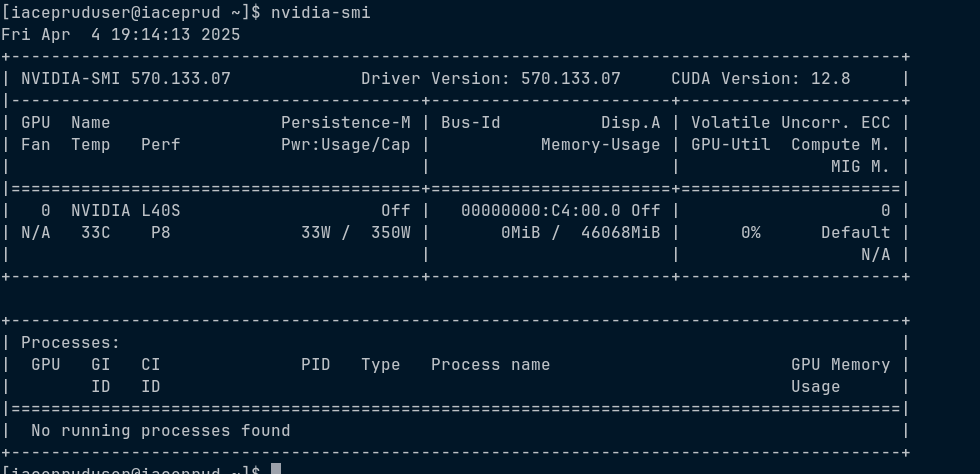
\includegraphics[width=1\textwidth]{imagenes/image6.png}
    \caption{Salida del comando nvidia-smi}
    \label{fig:nvidia-smi}
\end{figure}

Esta verificación confirmó la instalación de los \textit{NVIDIA Drivers 570}, compatibles con la gráfica, así como con \textit{CUDA 12.8}.

\section{Instalación de CUDA Toolkit}
Para la instalación del \textit{CUDA Toolkit}, se siguieron las instrucciones proporcionadas en el sitio oficial de \textit{NVIDIA}.~\cite{ref24} El proceso de instalación incluyó:
\begin{verbatim}
sudo dnf config-manager addrepo --from-repofile\ 
https://developer.download.nvidia.com/compute/cuda\
/repos/fedora41/x86_64/cuda-fedora41.repo
sudo dnf clean all
sudo dnf -y install cuda-toolkit-12-8
\end{verbatim}

Una vez instalado el \textit{CUDA Toolkit}, se configuraron las variables de entorno para asegurar que las herramientas de \textit{CUDA} fueran accesibles. Esto se realizó añadiendo las rutas a \texttt{~/.bashrc} y recargando el archivo:
\begin{verbatim}
echo 'export PATH=/usr/local/cuda/bin:$PATH' >> ~/.bashrc
echo 'export LD_LIBRARY_PATH=/usr/local/cuda/lib64:$LD_LIBRARY_PATH' >> ~/.bashrc
source ~/.bashrc
\end{verbatim}

Finalmente, se verificó la instalación del \textit{CUDA Toolkit} con:
\begin{verbatim}
nvcc --version
nvcc: NVIDIA (R) Cuda compiler driver
Copyright (c) 2005-2025 NVIDIA Corporation
Built on Fri_Feb_21_20:23:50_PST_2025
Cuda compilation tools, release 12.8, V12.8.93
Build cuda_12.8.r12.8/compiler.35583870_0
\end{verbatim}

Desde la perspectiva de los principios \textit{SRE}, este tipo de tarea representó mucho más que una simple instalación técnica; se trató de operar infraestructura con responsabilidad, bajo el principio de que fiabilidad y seguridad van de la mano. Con todo esto, se demostró que las acciones de personas con acceso privilegiado deben ser predecibles, auditables y reproducibles, lo cual aplicó incluso en tareas aparentemente rutinarias como esta. Concluido este proceso, el servidor disponía de las cualidades básicas necesarias para comenzar el despliegue de \textit{LLM} y servicios con \textit{OpenShift}.

\newpage
\section{Incidentes y Lecciones}
Tras completar la instalación de los controladores \textit{NVIDIA} y reiniciar el sistema con \texttt{sudo reboot}, el servidor no volvió a estar disponible. Aunque se intentó depurar el fallo mediante \texttt{ssh -vvv}, no se logró identificar el problema, y fue necesaria una intervención directa para recuperar la conexión con el servidor. Este incidente mostró cómo incluso acciones rutinarias como un reinicio pueden generar fallos críticos si no se ejecutan con las precauciones adecuadas.

También evidenció una debilidad común en entornos reales: la falta de mecanismos de visibilidad y trazabilidad inmediata ante un fallo. No contar con registros accesibles, métricas previas al apagado o algún tipo de diagnóstico automatizado complicó la identificación del origen del error y ralentizó la recuperación. Esto subrayó la importancia de contar con buenas prácticas de observabilidad y de preparar el entorno para análisis \textit{post-mortem}. %Definir un servicio Grafana sería una solución. 

Además, durante las prácticas \textit{Erasmus}, otro problema ocurrió cuando un compañero realizó una actualización en un servidor que tenía \textit{Secure Boot} activado. Esta función de seguridad del firmware \textit{UEFI} verifica que el software cargado al arrancar, como el sistema operativo y los controladores, esté firmado digitalmente por un proveedor de confianza. En este caso, al instalarse controladores no firmados, \textit{Secure Boot} bloqueó el arranque, dejando el sistema inutilizable. Gracias a que el rack estaba en la oficina, se pudo resolver físicamente, pero esta situación demostró cómo una configuración mal gestionada puede dejar fuera de servicio una máquina crítica, especialmente si no se tiene acceso físico inmediato o no se ha previsto un procedimiento de recuperación.

Estos eventos reflejaron la importancia de planificar operaciones sensibles como reinicios o actualizaciones: documentarlas, validarlas en entornos previos y prever escenarios de recuperación. En ingeniería de fiabilidad, pequeños errores operativos pueden comprometer la disponibilidad de todo el sistema, y por eso deben tratarse con el mismo rigor que los fallos de software o hardware.

